% This file was created with tikzplotlib v0.10.1.
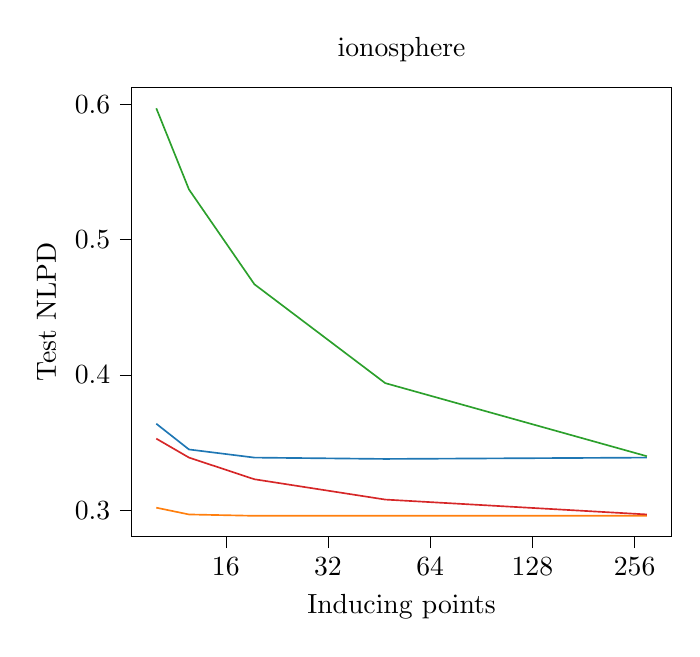
\begin{tikzpicture}

\definecolor{crimson2143940}{RGB}{214,39,40}
\definecolor{darkgray176}{RGB}{176,176,176}
\definecolor{darkorange25512714}{RGB}{255,127,14}
\definecolor{forestgreen4416044}{RGB}{44,160,44}
\definecolor{steelblue31119180}{RGB}{31,119,180}

\begin{axis}[
tick align=outside,
tick pos=left,
title={ionosphere},
x grid style={darkgray176},
xlabel={Inducing points},
xmin=4, xmax=268,
xtick style={color=black},
xtick={0,50,100,150,200,250,300},
xticklabels={0,16,32,64,128,256,},
y grid style={darkgray176},
ylabel={Test NLPD},
ymin=0.28095, ymax=0.61205,
ytick style={color=black}
]
\addplot [semithick, steelblue31119180]
table {%
16 0.364
32 0.345
64 0.339
128 0.338
256 0.339
};
\addplot [semithick, darkorange25512714]
table {%
16 0.302
32 0.297
64 0.296
128 0.296
256 0.296
};
\addplot [semithick, forestgreen4416044]
table {%
16 0.597
32 0.537
64 0.467
128 0.394
256 0.34
};
\addplot [semithick, crimson2143940]
table {%
16 0.353
32 0.339
64 0.323
128 0.308
256 0.297
};
\end{axis}

\end{tikzpicture}
